% Chapter Template

\chapter{Ensayos y resultados} % Main chapter title

\label{Chapter4} % Change X to a consecutive number; for referencing this chapter elsewhere, use \ref{ChapterX}

En este capítulo se presentan los resultados obtenidos en cada etapa del desarrollo de los modelos descrito en la sección~\ref{sec:desarrollo_modelos}. En primer lugar, se define el plan de evaluación: los conjuntos de datos, las métricas y las condiciones de comparación. A continuación, se presentan los resultados de cada etapa, que fundamentan las decisiones adoptadas en la siguiente, y se analizan los errores de la configuración seleccionada. Finalmente, se describen los ensayos del sistema integrado en producción.

%----------------------------------------------------------------------------------------
\section{Plan de evaluación}
\label{sec:plan_evaluacion}
%----------------------------------------------------------------------------------------

La evaluación tuvo como objetivo comparar los modelos en las mismas condiciones en las que operarían en producción. Por este motivo, los resultados de este capítulo se obtuvieron mediante el esquema de origen móvil presentado en la figura~\ref{fig:esquema_validacion}: en cada fecha de cálculo se utiliza solo la demanda observada hasta el día anterior y los pronósticos meteorológicos emitidos ese día, y los modelos se reentrenan periódicamente con todos los datos disponibles hasta ese momento.

Los datos utilizados comienzan el 01/01/2021. La tabla~\ref{tab:particion_datos} presenta los períodos que se utilizaron para cada propósito. El período de prueba no intervino en ninguna decisión de diseño: la selección de covariables, la búsqueda de hiperparámetros y la estimación de los umbrales de los grados-día utilizaron solo datos anteriores al 01/09/2025.

\begin{table}[H]
	\centering
	\caption{Períodos utilizados en el entrenamiento y la evaluación de los modelos.}
	\label{tab:particion_datos}
	\footnotesize
	\setlength{\tabcolsep}{4pt}
	\renewcommand{\arraystretch}{1.15}
	\begin{tabularx}{\textwidth}{
			@{}
			>{\raggedright\arraybackslash\hsize=0.6\hsize}X
			>{\raggedright\arraybackslash\hsize=1.0\hsize}X
			>{\raggedright\arraybackslash\hsize=1.4\hsize}X
			@{}
		}
		\toprule
		\textbf{Conjunto} & \textbf{Período} & \textbf{Uso} \\
		\midrule
		Entrenamiento & Desde el 01/01/2021 hasta el día anterior a cada reentrenamiento. & Ajuste de los modelos, con ventana creciente. \\
		Validación & Últimos 90 días previos a cada reentrenamiento. & Determinación de la cantidad de épocas de las redes neuronales. \\
		Validación & 01/09/2024 a 31/08/2025. & Selección de los grupos de covariables del modelo de referencia y búsqueda de hiperparámetros de LGBM\_OPT. \\
		Validación & 01/09/2023 a 31/08/2025. & Estimación de los umbrales de los grados-día. \\
		Prueba & 01/09/2025 a 31/08/2026. & Fechas de cálculo de todos los resultados de este capítulo. \\
		\bottomrule
	\end{tabularx}
\end{table}

\subsection{Métricas}
\label{subsec:metricas}

Se utilizaron las métricas definidas en la sección~\ref{sec:objetivos}: el error absoluto medio (MAE), la raíz del error cuadrático medio (RMSE) y el error porcentual absoluto medio (MAPE). Se agregó, además, el error porcentual medio, que mide el sesgo del pronóstico. Para un conjunto de $n$ pronósticos $\hat{y}_i$ con valores observados $y_i$, y con el error definido como $e_i = \hat{y}_i - y_i$, las métricas se calculan según las ecuaciones~\ref{eq:mae} a \ref{eq:sesgo}:

\begin{equation}
	\mathrm{MAE} = \frac{1}{n} \sum_{i=1}^{n} \left| e_i \right|
	\label{eq:mae}
\end{equation}

\begin{equation}
	\mathrm{RMSE} = \sqrt{\frac{1}{n} \sum_{i=1}^{n} e_i^{2}}
	\label{eq:rmse}
\end{equation}

\begin{equation}
	\mathrm{MAPE} = \frac{100}{n} \sum_{i=1}^{n} \left| \frac{e_i}{y_i} \right|
	\label{eq:mape}
\end{equation}

\begin{equation}
	\mathrm{Sesgo} = \frac{100}{n} \sum_{i=1}^{n} \frac{e_i}{y_i}
	\label{eq:sesgo}
\end{equation}

Un sesgo positivo indica que el modelo sobreestima la demanda, y uno negativo, que la subestima. El MAPE se adoptó como métrica principal, porque permite comparar variables y niveles de agregación de distinta magnitud y es la métrica habitual en el área de Programación Semanal y Diaria. El MAE y el RMSE se expresan en GWh para la energía y en MW para las potencias. El RMSE penaliza en mayor medida los errores grandes, por lo que su comparación con el MAE indica la presencia de días con errores elevados.

Las métricas se calculan por anticipación, de 0 a 14 días, y como promedio de todas las anticipaciones. En los gráficos, el MAPE se presenta en función de la anticipación, y la distribución del error porcentual de cada anticipación se representa mediante diagramas de caja, que muestran el sesgo y la dispersión de los errores.

\subsection{Alcance y condiciones de comparación}
\label{subsec:condiciones_comparacion}

Para acotar la extensión del capítulo, los resultados se presentan para el MEM. Las métricas de cada región eléctrica no se incluyen, aunque se calcularon con el mismo procedimiento y se encuentran disponibles en el sistema de monitoreo. En las configuraciones regionales, la energía del MEM se obtiene como suma de los pronósticos de las diez regiones, y se consideran solo las fechas en las que se dispone del pronóstico de todas ellas. Las potencias pico y mínima del MEM corresponden al pronóstico directo.

Los resultados se presentan por escenario meteorológico. El escenario con meteorología observada mide el error propio del modelo de demanda, mientras que el escenario con el pronóstico de IFS representa las condiciones de producción. IFS se adoptó como escenario principal porque es la única fuente con pronósticos de 15 días durante todo el período de prueba. ICON cubre solo las anticipaciones 0 a 6, y GFS está disponible desde el 02/04/2026. Por lo tanto, sus métricas no son comparables con las de los demás escenarios y solo se mencionan cuando aportan información adicional.

Dentro de cada escenario, los modelos se comparan sobre el mismo conjunto de fechas de cálculo y anticipaciones. Cuando se comparan escenarios entre sí, el conjunto se restringe además a las fechas disponibles en todos ellos. Por último, para analizar el desempeño en las condiciones más exigentes para la operación, se definen como días de alta demanda aquellos en los que la variable observada supera el percentil 90 de su distribución en el período de entrenamiento comprendido entre el 01/01/2021 y el 31/08/2025.

%----------------------------------------------------------------------------------------
\section{Evaluación del modelo}
\label{sec:evaluacion_modelo}
%----------------------------------------------------------------------------------------

Los resultados se presentan en el orden de las etapas descritas en la sección~\ref{sec:desarrollo_modelos}. Cada etapa se compara con la anterior, de modo que se identifique el aporte de cada decisión al desempeño final.

%----------------------------------------------------------------------------------------
\subsection{Modelo de referencia}
\label{subsec:resultados_referencia}
%----------------------------------------------------------------------------------------

La tabla~\ref{tab:resultados_referencia} presenta las métricas de la energía del MEM obtenidas por los modelos evaluados en la selección del modelo de referencia, con las covariables del día pronosticado. LightGBM y XGBoost obtuvieron los menores errores, con resultados prácticamente equivalentes: con la meteorología observada, el MAPE fue de 2,37\,\% y 2,42\,\%, respectivamente, y con el pronóstico de IFS, de 4,66\,\% y 4,60\,\%. Random Forest presentó errores algo mayores, mientras que la regresión lineal presentó un MAPE superior al 7\,\% en ambos escenarios, cercano al del modelo ingenuo estacional. Este resultado indica que la relación entre la demanda y sus covariables no se representa adecuadamente con una combinación lineal, aun con los cuadrados de las temperaturas.

\begin{table}[H]
	\centering
	\caption{Métricas de la energía del MEM de los modelos evaluados en la selección del modelo de referencia, promedio de las anticipaciones 0 a 14. MAPE y sesgo en \%, RMSE en GWh.}
	\label{tab:resultados_referencia}
	\footnotesize
	\setlength{\tabcolsep}{4pt}
	\renewcommand{\arraystretch}{1.15}
	\begin{tabular}{@{}lcccccc@{}}
		\toprule
		& \multicolumn{3}{c}{\textbf{Meteorología observada}} & \multicolumn{3}{c}{\textbf{Pronóstico IFS}} \\
		\cmidrule(lr){2-4} \cmidrule(l){5-7}
		\textbf{Modelo} & \textbf{MAPE} & \textbf{RMSE} & \textbf{Sesgo} & \textbf{MAPE} & \textbf{RMSE} & \textbf{Sesgo} \\
		\midrule
		LightGBM & 2,37 & 12,4 & $-1{,}44$ & 4,66 & 27,0 & $-0{,}80$ \\
		XGBoost & 2,42 & 12,9 & $-1{,}38$ & 4,60 & 26,8 & $-0{,}75$ \\
		Random Forest & 2,89 & 15,3 & $-1{,}22$ & 4,84 & 27,8 & $-0{,}58$ \\
		Regresión lineal & 7,79 & 38,6 & $-0{,}80$ & 8,20 & 41,1 & $-0{,}52$ \\
		SNAIVE & 9,14 & 48,2 & 0,66 & 9,15 & 48,2 & 0,71 \\
		\bottomrule
	\end{tabular}
\end{table}

La figura~\ref{fig:referencia_mape} muestra el MAPE en función de la anticipación. Con la meteorología observada, el error de los modelos basados en árboles aumenta entre la anticipación~0 y la~1 y luego se mantiene casi constante, con un MAPE de LightGBM de 1,76\,\% en el día~0 y de 2,52\,\% en el día~14. Con el pronóstico de IFS, en cambio, el error crece en forma sostenida con la anticipación, desde 2,11\,\% hasta 7,79\,\%. La diferencia entre ambos escenarios muestra que, a partir de los primeros días, el error del pronóstico meteorológico supera al error propio del modelo de demanda y determina la evolución del error con el horizonte. Estos valores se ubican en el rango que documentaban las evaluaciones internas de CAMMESA, de aproximadamente 3\,\% para el día siguiente y 10\,\% para los horizontes más alejados, mencionadas en la sección~\ref{sec:estado_arte}.

\begin{figure}[H]
	\centering
	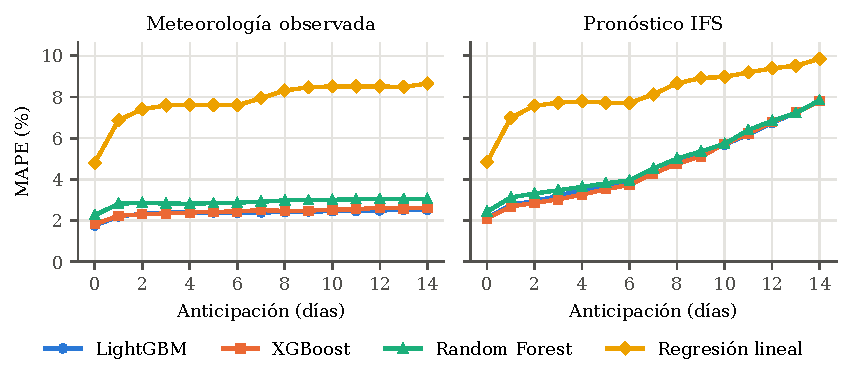
\includegraphics[width=\textwidth]{./Figures/cap4_referencia_mape.pdf}
	\caption{MAPE de la energía del MEM por anticipación de los modelos evaluados en la selección del modelo de referencia.}
	\label{fig:referencia_mape}
\end{figure}

La figura~\ref{fig:referencia_sesgo} presenta la distribución del error porcentual de LightGBM con el pronóstico de IFS. La mediana se mantiene cerca de cero en todo el horizonte, con una leve tendencia a la subestimación, mientras que la dispersión aumenta con la anticipación. El intervalo entre los percentiles 5 y 95 pasa de $-4{,}9$\,\% a 3,9\,\% en el día~0 a $-17{,}2$\,\% a 16,1\,\% en el día~14.

\begin{figure}[H]
	\centering
	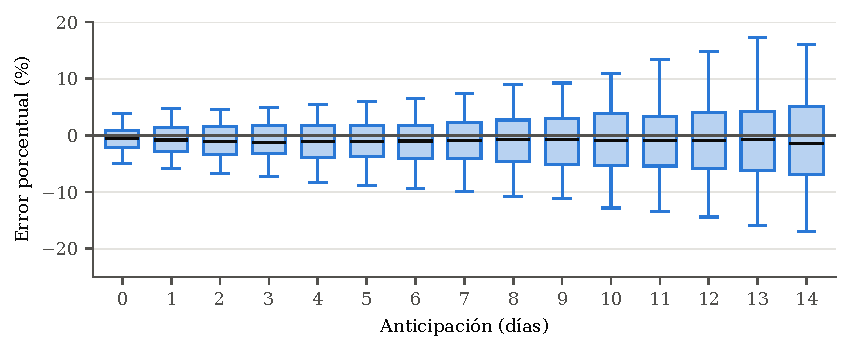
\includegraphics[width=\textwidth]{./Figures/cap4_referencia_sesgo.pdf}
	\caption{Distribución del error porcentual de la energía del MEM por anticipación de LightGBM con el pronóstico de IFS. Las cajas representan los percentiles 25 y 75, y los bigotes, los percentiles 5 y 95.}
	\label{fig:referencia_sesgo}
\end{figure}

La variante que incorpora las covariables de los días anteriores al pronosticado no modificó el desempeño de los modelos basados en árboles. El MAPE de LightGBM fue de 2,29\,\% con la meteorología observada y de 4,67\,\% con IFS, frente a 2,37\,\% y 4,66\,\% sin esas covariables. La regresión lineal mejoró, de 7,79\,\% a 7,17\,\% con la meteorología observada, aunque sin alcanzar a los demás modelos. Por lo tanto, se mantuvo la formulación con las covariables del día pronosticado, que es más simple. Entre LightGBM y XGBoost, se eligió LightGBM como modelo de referencia por su menor costo de entrenamiento, ya que su desempeño fue equivalente.

%----------------------------------------------------------------------------------------
\subsection{Modelos de aprendizaje profundo y fundacionales}
\label{subsec:resultados_profundos}
%----------------------------------------------------------------------------------------

La tabla~\ref{tab:resultados_profundos} presenta las métricas de la energía del MEM obtenidas en la segunda etapa. En esta etapa, la historia de pronósticos de IFS disponible cubría las anticipaciones 0 a 12, por lo que las métricas de ese escenario corresponden a ese rango. La tabla incluye el tiempo medio de cada reentrenamiento mensual de los modelos entrenados con GPU.

\begin{table}[H]
	\centering
	\caption{Métricas de la energía del MEM de los modelos de aprendizaje profundo y fundacionales, y tiempo medio de entrenamiento. MAPE y sesgo en \%, RMSE en GWh y tiempo en segundos.}
	\label{tab:resultados_profundos}
	\footnotesize
	\setlength{\tabcolsep}{4pt}
	\renewcommand{\arraystretch}{1.15}
	\begin{tabular}{@{}lcccccc@{}}
		\toprule
		& \multicolumn{2}{c}{\textbf{Meteorología observada}} & \multicolumn{3}{c}{\textbf{Pronóstico IFS}} & \\
		\cmidrule(lr){2-3} \cmidrule(lr){4-6}
		\textbf{Modelo} & \textbf{MAPE} & \textbf{RMSE} & \textbf{MAPE} & \textbf{RMSE} & \textbf{Sesgo} & \textbf{Tiempo} \\
		\midrule
		TSMixer & 1,63 & 8,6 & 3,93 & 23,0 & 0,16 & 98 \\
		TFT & 1,79 & 9,6 & 4,10 & 23,6 & 0,00 & 634 \\
		GRU & 1,85 & 10,1 & 3,99 & 23,4 & 0,16 & 24 \\
		LSTM & 1,90 & 10,1 & 3,97 & 23,2 & $-0{,}04$ & 24 \\
		LGBM\_OPT & 2,29 & 11,8 & 4,14 & 24,0 & $-0{,}85$ & -- \\
		TiDE & 2,32 & 12,0 & 4,20 & 24,0 & $-0{,}21$ & 80 \\
		LightGBM & 2,39 & 12,7 & 4,22 & 24,3 & $-0{,}88$ & -- \\
		Chronos-2 ajustado & 2,99 & 15,3 & 4,70 & 25,8 & 0,17 & 338 \\
		Chronos-2 sin ajuste & 3,55 & 18,9 & 4,98 & 27,3 & $-0{,}53$ & -- \\
		SNAIVE & 9,14 & 48,2 & 8,99 & 47,5 & 0,71 & -- \\
		\bottomrule
	\end{tabular}
\end{table}

Con la meteorología observada, todas las redes neuronales superaron al modelo de referencia, aunque TiDE quedó muy cerca. TSMixer obtuvo el menor error, con un MAPE de 1,63\,\%, un 29\,\% inferior al de LGBM\_OPT. Con el pronóstico de IFS, las diferencias se reducen: los modelos entrenados, salvo Chronos-2, se ubican entre 3,93\,\% y 4,22\,\%, porque el error del pronóstico meteorológico, común a todos, pasa a dominar. El ajuste de hiperparámetros de LightGBM produjo una mejora pequeña, de 2,39\,\% a 2,29\,\% con la meteorología observada y de 4,22\,\% a 4,14\,\% con IFS.

La figura~\ref{fig:profundos_mape} muestra el comportamiento por anticipación de los modelos más representativos de cada familia. Con la meteorología observada, el error de TSMixer, que genera el horizonte completo en un único paso, se mantiene casi constante, entre 1,45\,\% y 1,71\,\%. Las redes recurrentes, en cambio, obtienen el menor error en el día~0, con 1,19\,\% en LSTM, pero su error crece con la anticipación hasta 2,27\,\% en el día~14, como consecuencia de la acumulación de errores de la estrategia recursiva. Con IFS, las curvas de todos los modelos entrenados prácticamente se superponen a partir del día~7.

\begin{figure}[H]
	\centering
	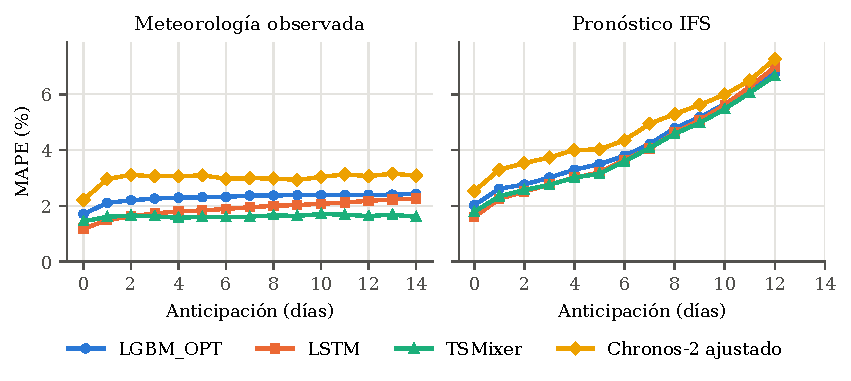
\includegraphics[width=\textwidth]{./Figures/cap4_profundos_mape.pdf}
	\caption{MAPE de la energía del MEM por anticipación de modelos seleccionados de la segunda etapa.}
	\label{fig:profundos_mape}
\end{figure}

La figura~\ref{fig:profundos_sesgo} compara la distribución del error porcentual de LGBM\_OPT y TSMixer con IFS. LGBM\_OPT presenta una mediana negativa en casi todo el horizonte, que confirma la tendencia del modelo de referencia a subestimar la demanda. TSMixer tiene un sesgo cercano a cero y una dispersión menor en las primeras anticipaciones. En el día~12, ambos modelos presentan una dispersión similar, con un percentil 5 cercano a $-14$\,\% y un percentil 95 de entre 15\,\% y 17\,\%.

\begin{figure}[H]
	\centering
	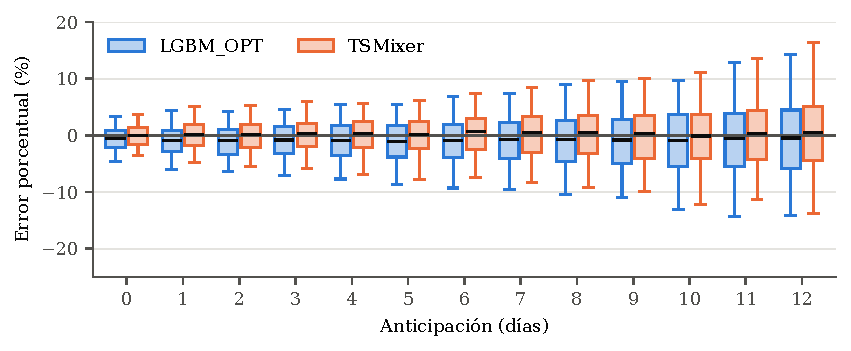
\includegraphics[width=\textwidth]{./Figures/cap4_profundos_sesgo.pdf}
	\caption{Distribución del error porcentual de la energía del MEM por anticipación de LGBM\_OPT y TSMixer con el pronóstico de IFS. Las cajas representan los percentiles 25 y 75, y los bigotes, los percentiles 5 y 95.}
	\label{fig:profundos_sesgo}
\end{figure}

Chronos-2 obtuvo los mayores errores entre los modelos entrenados. El ajuste mediante LoRA redujo su MAPE de 3,55\,\% a 2,99\,\% con la meteorología observada, pero no alcanzó al modelo de referencia, con un costo de entrenamiento superior al de las redes recurrentes y TSMixer. TiDE tuvo un desempeño inferior a TSMixer, la otra arquitectura basada en perceptrones multicapa, y TFT obtuvo resultados cercanos a los de TSMixer con un tiempo de entrenamiento seis veces mayor. A partir de estos resultados, se mantuvieron para las etapas siguientes los modelos indicados en la sección~\ref{subsec:covariables_agregacion}.

%----------------------------------------------------------------------------------------
\subsection{Covariables, fuentes meteorológicas y nivel de agregación}
\label{subsec:resultados_covariables}
%----------------------------------------------------------------------------------------

La tabla~\ref{tab:resultados_g5} compara las configuraciones Regional G5, Regional G5A y MEM G5 en la energía del MEM. En esta etapa se incorporaron los ensambles.

\begin{table}[H]
	\centering
	\caption{MAPE (\%) de la energía del MEM según la configuración, promedio de las anticipaciones 0 a 14. G5 y G5A corresponden a las configuraciones regionales.}
	\label{tab:resultados_g5}
	\footnotesize
	\setlength{\tabcolsep}{4pt}
	\renewcommand{\arraystretch}{1.15}
	\begin{tabular}{@{}lcccccc@{}}
		\toprule
		& \multicolumn{3}{c}{\textbf{Meteorología observada}} & \multicolumn{3}{c}{\textbf{Pronóstico IFS}} \\
		\cmidrule(lr){2-4} \cmidrule(l){5-7}
		\textbf{Modelo} & \textbf{G5} & \textbf{G5A} & \textbf{MEM G5} & \textbf{G5} & \textbf{G5A} & \textbf{MEM G5} \\
		\midrule
		ENS\_STACK & 1,42 & 1,63 & 1,87 & 4,39 & 4,70 & 4,58 \\
		ENS\_PROM & 1,51 & 1,70 & 2,44 & 4,29 & 4,58 & 4,70 \\
		TSMixer & 1,57 & 1,86 & 3,37 & 4,33 & 4,64 & 5,34 \\
		GRU & 1,67 & 2,11 & 2,28 & 4,37 & 4,82 & 4,68 \\
		TFT & 1,68 & 1,69 & 3,25 & 4,51 & 4,73 & 5,18 \\
		LSTM & 1,82 & 1,84 & 2,83 & 4,43 & 4,57 & 4,85 \\
		LGBM\_OPT & 2,29 & 2,20 & 2,64 & 4,59 & 4,83 & 4,80 \\
		SNAIVE & 9,14 & 9,14 & 9,14 & 9,15 & 9,15 & 9,15 \\
		\bottomrule
	\end{tabular}
\end{table}

Los ensambles mejoraron a los modelos individuales con la meteorología observada. ENS\_STACK obtuvo un MAPE de 1,42\,\%, inferior al 1,57\,\% de TSMixer, el mejor modelo individual. Con IFS, ENS\_PROM y ENS\_STACK quedaron cerca del mejor modelo individual, con 4,29\,\% y 4,39\,\%, ya que el error meteorológico afecta a todos los modelos de la misma forma y reduce el beneficio de combinarlos.

La temperatura del aire produjo errores mayores que la temperatura aparente en casi todos los modelos. El MAPE de ENS\_STACK aumentó de 1,42\,\% a 1,63\,\% con la meteorología observada y de 4,39\,\% a 4,70\,\% con IFS. La temperatura aparente incorpora el efecto de la humedad y del viento sobre la sensación térmica, que influye en el uso de equipos de climatización. Por este motivo, se mantuvo como opción principal.

El pronóstico directo de la energía del MEM resultó menos preciso que la suma de los pronósticos regionales en todos los modelos, con un MAPE de ENS\_STACK de 1,87\,\% frente a 1,42\,\% con la meteorología observada. Las diferencias fueron mayores en TSMixer y TFT, que en el pronóstico directo disponen de una única serie para entrenar, en lugar de las diez series regionales del entrenamiento global. Por lo tanto, la energía del MEM se obtiene como suma de las regiones.

\subsubsection{Grupos de pronósticos}

La figura~\ref{fig:grupos_mape} compara el MAPE de ENS\_STACK en la configuración Regional G5A con el pronóstico de IFS y con los dos grupos de pronósticos de la tabla~\ref{tab:grupos_pronosticos}. Los grupos redujeron el MAPE promedio de 4,60\,\% con IFS a 4,06\,\% con TWC + IFS y a 4,09\,\% con SMN + TWC + IFS, sobre el mismo conjunto de fechas. La mejora se concentra en las anticipaciones mayores: en el día~14, el MAPE pasa de 7,57\,\% con IFS a 6,35\,\% con TWC + IFS. Con ambos grupos, la configuración Regional G5A superó también el resultado de Regional G5 con IFS, de 4,39\,\%. Es decir, la menor precisión de la temperatura del aire se compensa con la combinación de fuentes que esa variable permite.

\begin{figure}[H]
	\centering
	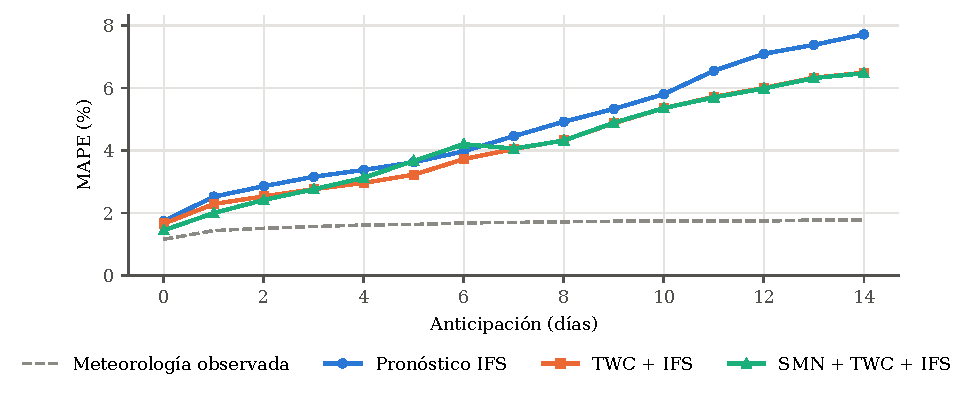
\includegraphics[width=\textwidth]{./Figures/cap4_grupos_mape.pdf}
	\caption{MAPE de la energía del MEM por anticipación de ENS\_STACK en la configuración Regional G5A, según el pronóstico meteorológico utilizado.}
	\label{fig:grupos_mape}
\end{figure}

El pronóstico del SMN mejoró las tres primeras anticipaciones, con un MAPE de 1,46\,\% en el día~0 frente a 1,66\,\% con TWC, pero empeoró las anticipaciones 4 a 6, en las que alcanzó 4,07\,\% en el día~6 frente a 3,62\,\%. En promedio, no mejoró al grupo que prescinde de esa fuente. Por este motivo, se adoptó el grupo TWC + IFS.

\subsubsection{Indicador de actividad económica}

La incorporación del EMAE produjo resultados dispares. Con la meteorología observada, el MAPE de LSTM se redujo de 1,90\,\% a 1,71\,\% y el de LGBM\_OPT, de 2,29\,\% a 2,05\,\%, mientras que el de TSMixer aumentó de 1,63\,\% a 1,87\,\%. Con IFS, las variaciones fueron de hasta 0,2 puntos porcentuales, en ambos sentidos. La ausencia de una mejora consistente, sumada al costo de mantener una fuente externa adicional, fundamentó la decisión de no incorporarlo.

\subsubsection{Potencias del MEM y comparación con el modelo de producción}

La tabla~\ref{tab:resultados_mem_g5} presenta las métricas de la configuración MEM G5 para las tres variables objetivo

\begin{table}[H]
	\centering
	\caption{MAPE (\%) de la configuración MEM G5 por variable objetivo, promedio de las anticipaciones 0 a 14.}
	\label{tab:resultados_mem_g5}
	\footnotesize
	\setlength{\tabcolsep}{4pt}
	\renewcommand{\arraystretch}{1.15}
	\begin{tabular}{@{}lcccccc@{}}
		\toprule
		& \multicolumn{3}{c}{\textbf{Meteorología observada}} & \multicolumn{3}{c}{\textbf{Pronóstico IFS}} \\
		\cmidrule(lr){2-4} \cmidrule(l){5-7}
		\textbf{Modelo} & \textbf{EN} & \textbf{PI} & \textbf{MI} & \textbf{EN} & \textbf{PI} & \textbf{MI} \\
		\midrule
		ENS\_STACK & 1,87 & 2,24 & 2,07 & 4,58 & 5,26 & 4,27 \\
		ENS\_PROM & 2,44 & 2,78 & 2,26 & 4,70 & 5,41 & 4,25 \\
		GRU & 2,28 & 2,69 & 2,47 & 4,68 & 5,49 & 4,41 \\
		LGBM\_OPT & 2,64 & 3,00 & 2,85 & 4,80 & 5,46 & 4,56 \\
		LSTM & 2,83 & 3,27 & 2,64 & 4,85 & 5,65 & 4,64 \\
		TFT & 3,25 & 3,31 & 2,64 & 5,18 & 5,89 & 4,58 \\
		TSMixer & 3,37 & 3,35 & 3,11 & 5,34 & 5,83 & 4,72 \\
		RLIN\_LEGACY & 6,08 & 5,91 & 5,35 & 7,41 & 7,51 & 6,44 \\
		SNAIVE & 9,14 & 9,72 & 8,68 & 9,15 & 9,72 & 8,67 \\
		\bottomrule
	\end{tabular}
\end{table}

ENS\_STACK obtuvo el menor error en las tres variables. La potencia pico resultó la variable más difícil de pronosticar, con un MAPE de 5,26\,\% con IFS, ya que corresponde a un valor horario extremo, mientras que la energía integra el comportamiento de todo el día. Respecto de RLIN\_LEGACY (la réplica de la regresión lineal utilizada en producción antes del trabajo), el MAPE con IFS se redujo un 30\,\% en la potencia pico y un 34\,\% en la potencia mínima. En la energía, la reducción alcanza el 41\,\% si se considera la suma de los pronósticos regionales de la configuración Regional G5, con un MAPE de 4,39\,\% frente a 7,41\,\%.

%----------------------------------------------------------------------------------------
% PENDIENTE: resultados de las etapas restantes y secciones siguientes
%----------------------------------------------------------------------------------------
% 4.2.4 Representación de la respuesta a la temperatura (Regional G6, G6A, MEM G6, MEM G6A;
%       LGBM_OPT_PESOS; días de alta demanda).
% 4.2.5 Corrección y combinación de los pronósticos (MOS, híbridos, promedio de fuentes,
%       corrección del sesgo reciente; resultado final para EN, PI y MI).
% 4.3   Análisis de errores (días de alta demanda, estaciones del año, feriados, casos límite).
% 4.4   Ensayos de integración del sistema (ejecución diaria, tiempos, monitoreo en Power BI).
